\section{40-bit One-Max with FGR and FP}

Chosing a good fitness function was paramount in minimizing the needed population size. A punishing one was chosen (fitness proportionate with the inverse of the error), which greatly increased the effectiveness of fitness-proportionate scaling due to greater spacing of good phenotypes.

A population size of 80 was consistently able to terminate in 100 generations or less (52 generations average, standard deviation 12.61, 100 runs sample size).

A per bit mutation chance of $(0.01 > \epsilon > 0.001)$ and a crossover rate of $ \epsilon > 0.9 $ was found to be optimal. Higher mutation chances led to randomized search, the opposite causing stagnation of the gene pool due to cycles and lack of variance. If none of the genomes have bit $n$ set, no amount of crossover can generate a solution. Fitness graphs a to c in figure \ref{fig:fgp-fp-fitness-graphs} illustrate these findings.

\begin{figure}[H]
        \centering
        \begin{subfigure}[b]{0.5\textwidth}
                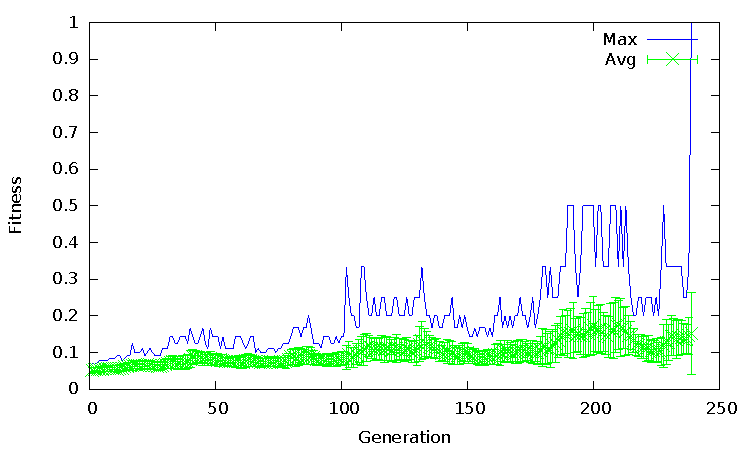
\includegraphics[width=\textwidth]{../results/omx-fgr-fp/omx-80-06-003.pdf}
                \caption{Generation size 80, crossover chance 0.6, mutation chance 0.03}
                \label{fig:gull}
        \end{subfigure}%
        \begin{subfigure}[b]{0.5\textwidth}
                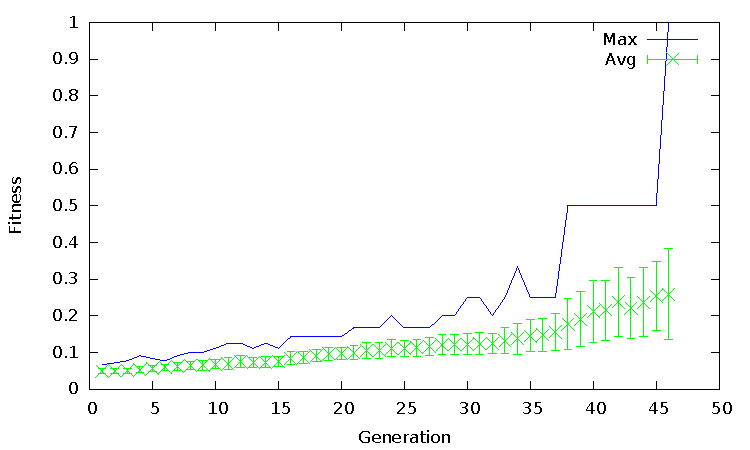
\includegraphics[width=\textwidth]{../results/omx-fgr-fp/omx-80-1-001.pdf}
                \caption{Generation size 80, crossover chance 1, mutation chance 0.01}
                \label{fig:tiger}
        \end{subfigure}
        \begin{subfigure}[b]{0.5\textwidth}
                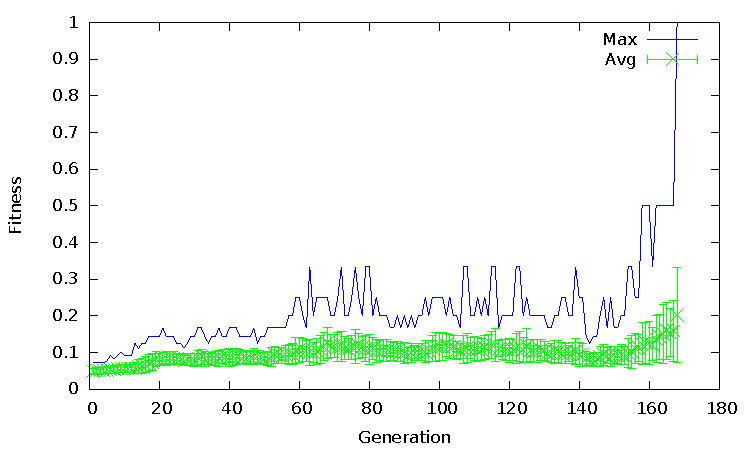
\includegraphics[width=\textwidth]{../results/omx-fgr-fp/omx-80-1-003.pdf}
                \caption{Generation size 80, crossover chance 1, 0.03 mutation chance}
                \label{fig:mouse}
        \end{subfigure}%
		\begin{subfigure}[b]{0.5\textwidth}
			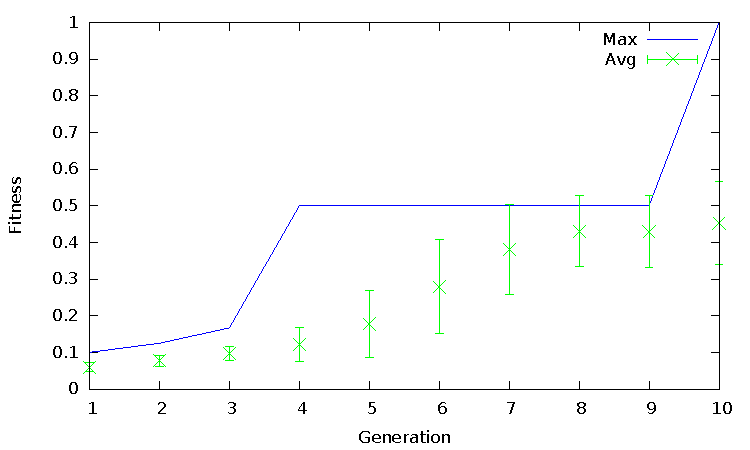
\includegraphics[width=\textwidth]{../results/40-random/random-with-tournament.pdf}
			\caption{Finding a random 40-length bit vector with tournament selection}
			\label{fig:random-tournament}
		\end{subfigure}
        \caption{Different parameters for FGR and FP (Includes orphaned figure for section \ref{sec:modified-vector} due to space issues)}
        \label{fig:fgp-fp-fitness-graphs}
\end{figure}